\documentclass[../main.tex]{subfiles}

\begin{document}
\begin{CJK*}{UTF8}{gbsn}

\section*{Exercice 3d}
On compare deux estimateurs de la fonction de risque et produire deux graphiques séparés.
\begin{enumerate}
1. Il représente la fonction $h^\hat{(t)} = \frac{d_i}{n_i}$, l'intervalle de temps est $t$ entre 200 et 260.\
2. Il montre la fonction $h^\hat{(t)}$ lissée avec le noyau d'Epanechnikov, également pour $t$ entre 200 et 260.
\end{enumerate}



\begin{lstlisting}
#3d
debut <- 200
fin <- 260

p <- ggplot(data.frame(t = t[debut:fin], q = q[debut:fin]), aes(x = t, y = q)) +
  geom_line() +  labs(title = "Line Chart Example", x = "Time", y = "Value")
show(p)

epanechnikov <- function(u) {
  if (abs(u) <= 1) {
    return(0.75 * (1 - u^2))
  } else {
    return(0)
  }
}

b <- 5
D <- length(t[sort(time_days[event == 1])])
lisse <- rep(0, fin - debut)
for (i in debut:fin) {
  diff_seq <- (i - t[sort(time_days[event == 1])])/b
  epan <- rep(0, D)
  for (j in 1:D) {
    epan[j] <- epanechnikov(diff_seq[j])
  }
  lisse[i - debut + 1] <- (1/b)*sum(q[sort(time_days[event == 1])] * epan)
}

p <- ggplot(data.frame(t = t[debut:fin], lisse = lisse), aes(x = t, y = lisse)) +
  geom_line() +  labs(title = "Line Chart Example", x = "Time", y = "Value")
show(p)

\end{lstlisting}

\begin{figure}[H]
  \centering
  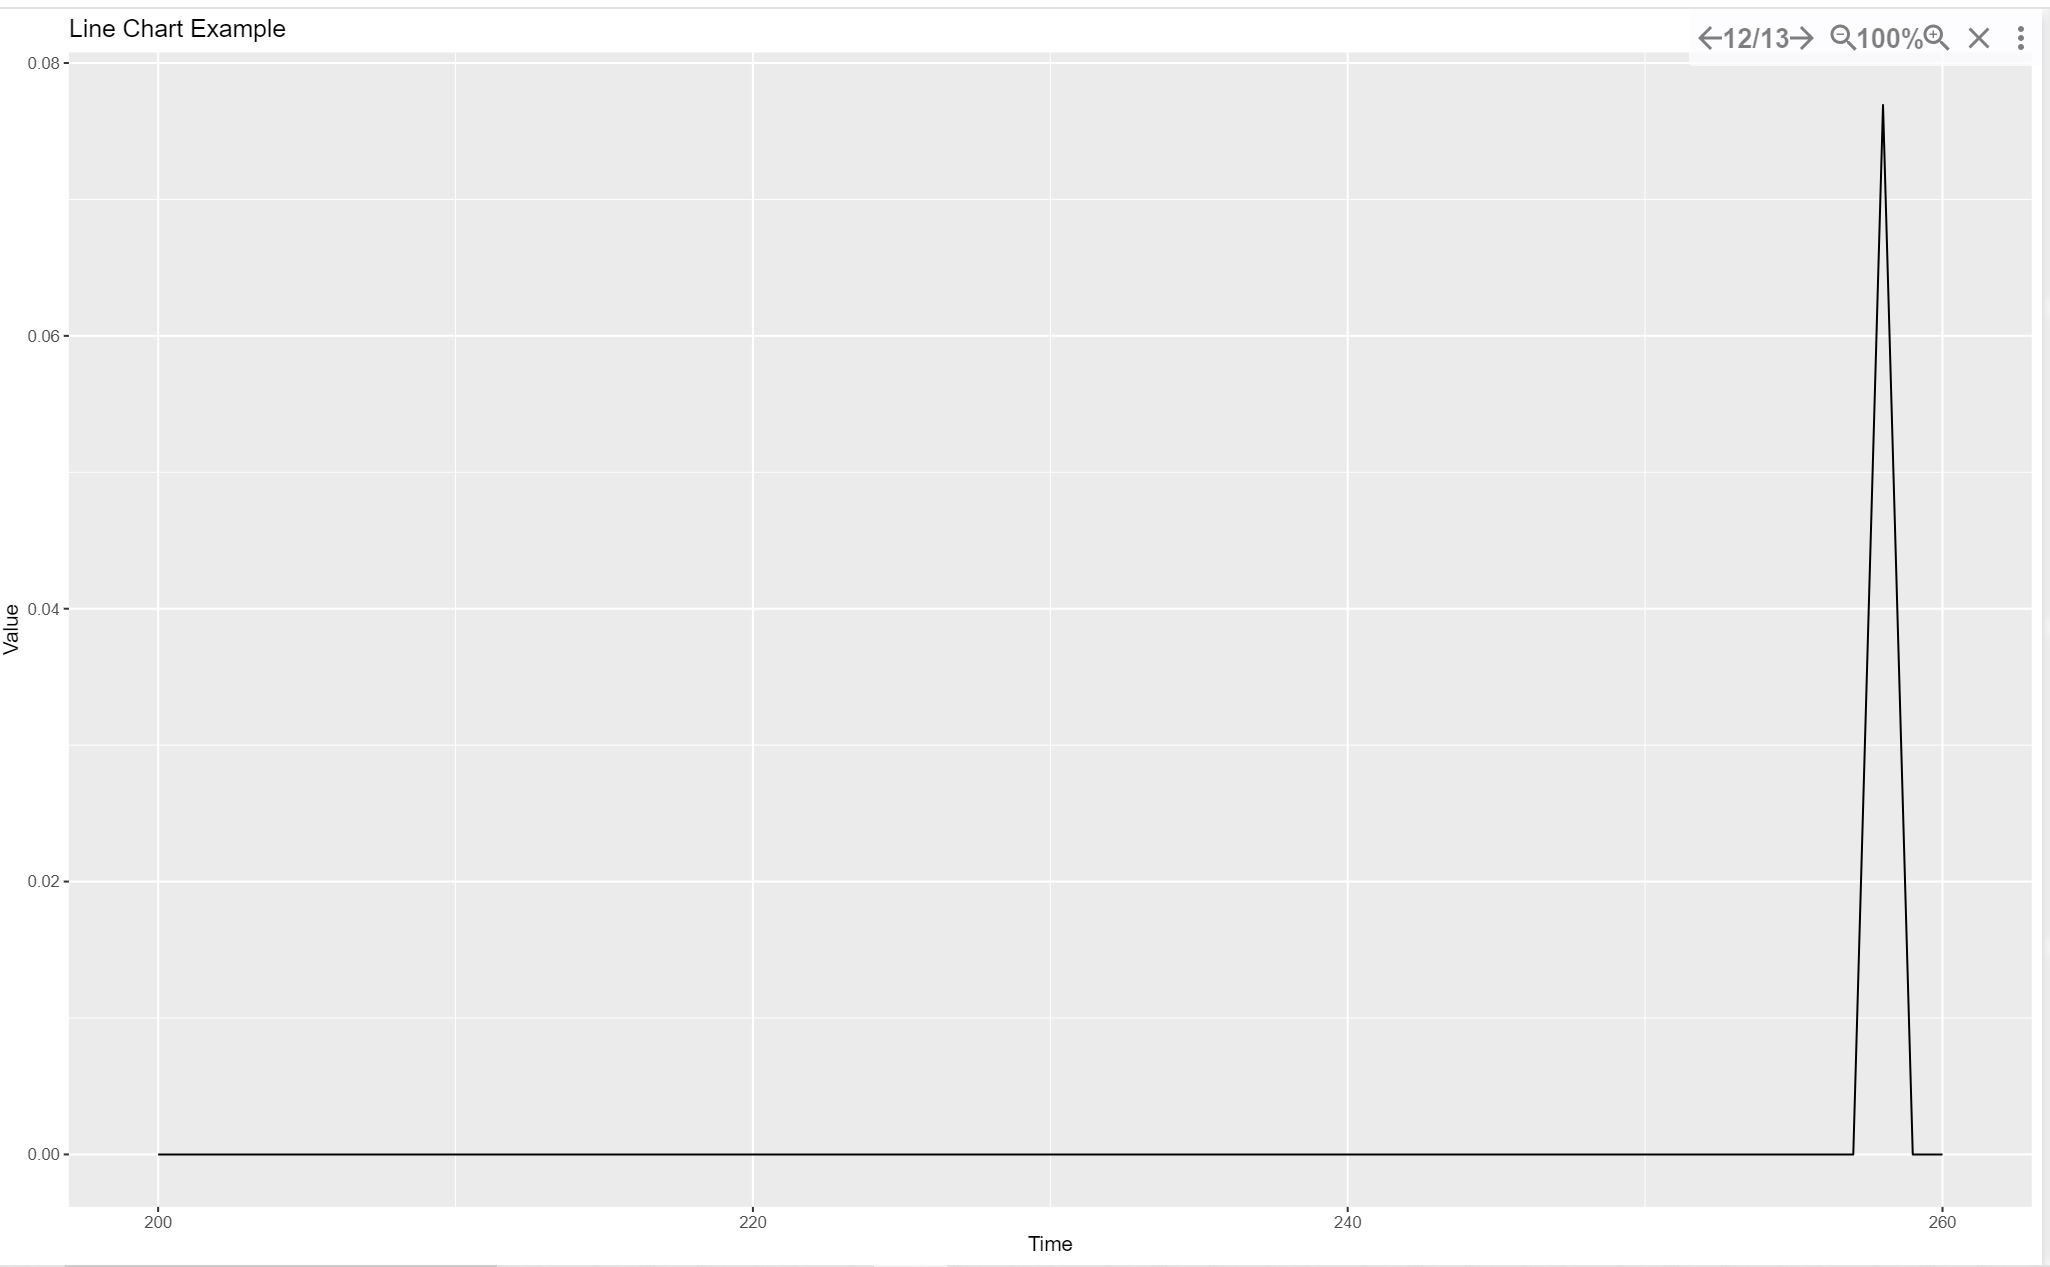
\includegraphics[width=0.8\textwidth]{3D2.JPG}
  \label{fig:mesh1}
\end{figure}

\begin{figure}[H]
  \centering
  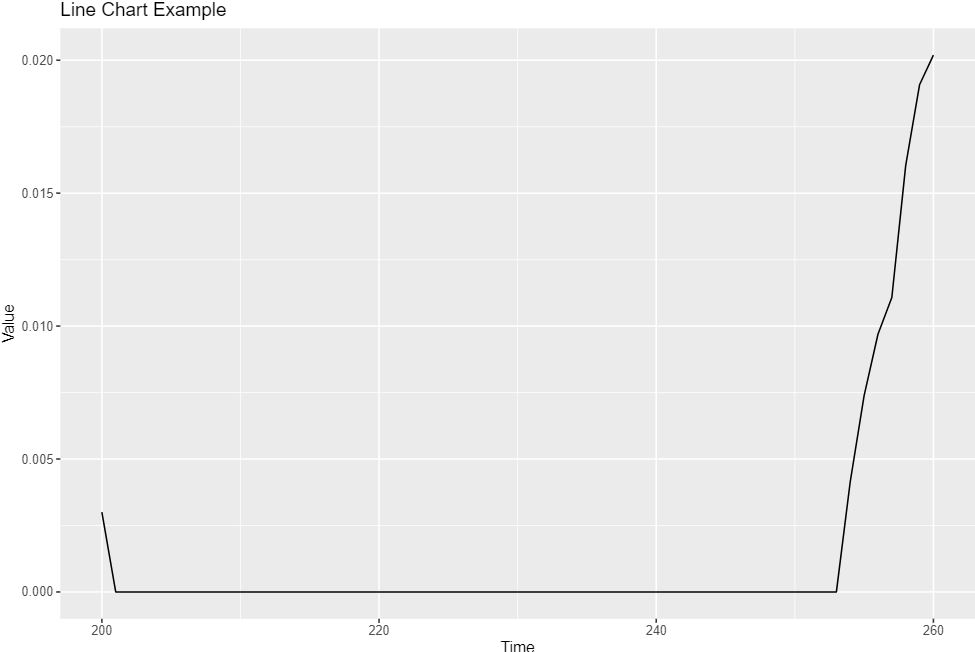
\includegraphics[width=0.8\textwidth]{3D.JPG}
  \label{fig:mesh1}
\end{figure}



\end{CJK*}
\end{document}
